%% Autor: Björn Ritterbecks 
%% Letzte Aenderung: 15.06.2016 
\thisfloatsetup{%
  capbesidewidth=\marginparwidth}
\begin{figure}[htbp]
\vspace*{0.2cm}
\centering
%\sansmath
 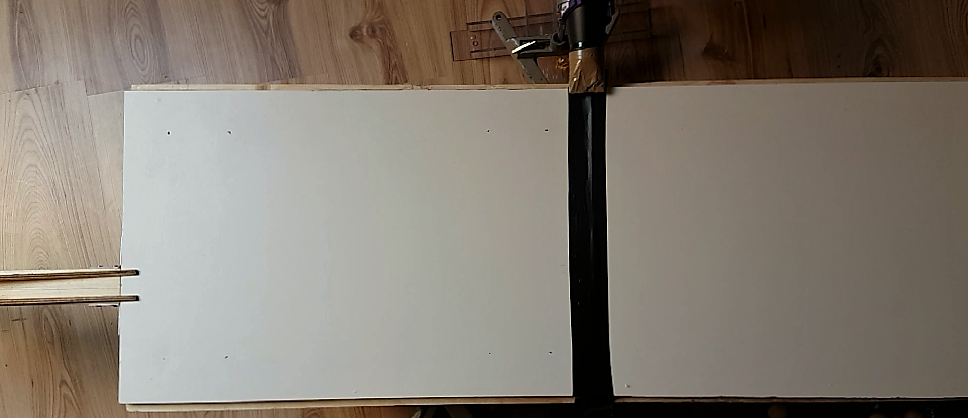
\includegraphics[width=0.99\textwidth]{images/Aufbau.png}
  \caption[Versuchsaufbau ohne Detektoren]{Fotografie des Versuchsaufbaus ohne Detektoren. Bei der linken Platte handelt es sich um die schiefe Ebene. Das Gebläse wirkt mit der höchsten Kraft im Übergangsbereich der beiden Platten. Durch die Aufhängung mit Winkeln kann die Rampe auch näher am Gebläse positioniert werden.}
  \label{fig:aufbau1}
  \vspace{-0pt}
\end{figure}